\documentclass[spanish]{udpreport}
\usepackage[utf8]{inputenc}
\usepackage[spanish]{babel}
\usepackage{graphicx} % figuras
\usepackage{subfigure} 
\usepackage{subfig}

% Podemos establecer el logo de alguna entidad o dejar el de la UDP (defecto)
%\setlogo{EITFI}

\title{Comprobación del funcionamiento del algoritmo STP e implementación de VLAN\\Laboratorio 4, Redes de datos}
\author{Integrantes: Luis Canales, Nicolás Flores, Christian López, Bastián López.\\Profesor: Jaime Álvarez \\ Ayudante: Maximiliano Vega}

\date{14 de Mayo de 2016}

% Además podemos establecer la facultad y escuela
% los valores por defecto son los siguientes:
%\udpschool{Escuela de Informática y Telecomunicaciones}
%\udpfaculty{Facultad de Ingeniería}
%\udpuniversity{Universidad Diego Portales}

\begin{document}
\maketitle

\tableofcontents

\chapter{Introducción}
Como sabemos, tener una red optimizada, es fundamental en una organización, ya que esta puede ser un factor determinante en la productividad y reputación al momento de realizar sus transmisiones en forma prevista, una tecnología que puede mejorar notablemente el rendimiento de una red, son las VLAN  estas se pueden definir como subredes independientes de área local que agrupan un conjunto de dispositivos de manera lógica y no física. Algunas de las múltiples ventajas que poseen es que son útiles para disminuir el dominio de difusión y ayudan a la administración de la red, separando segmentos lógicos de una red de área local, que no deberían intercambiar datos usando la red local.

Por otra parte, el protocolo STP es un protocolo que tiene como principal objetivo, encargarse de mantener una red libre de bucles en trayectos redundantes en la red. Los bucles son fatales para una red.\\
En este laboratorio levantamos diferentes topologías de redes que presentaban bucles para poder analizar el funcionamiento del algoritmo Spanning Tree Protocol (STP). Además configuramos diferentes dispositivos para que pudieran estar conectados a diferentes VLANs.\\
Para realizar las actividades propuestas debimos utilizar el programa Packet Tracer, el cual sirve para poder crear redes y configurar el funcionamiento de cada equipo creado. \\


\section{STP: Spanning Tree Protocol}
\begin{itemize}
\item
El protocolo STP (Spanning Tree Protocol), el cual posee la especificación IEEE 802.1D, es un protocolo de red de nivel dos del modelo OSI, el objetivo de este protocolo, es mantener una red libre de bucles. Un camino libre de bucles se consigue cuando un dispositivo es capaz de reconocer un bucle en la topología y bloquea uno o más puertos redundantes. Este protocolo explora constantemente la red, de modo que cualquier fallo o adición en un enlace, Switch o Bridge, es detectado inmediatamente, ya que por lo contrario, si una red posee un bucle, esta presentaría múltiples problemas, como puede ser el caso que los paquetes enviados que podrían llegar más de una vez al mismo destino.


\end{itemize}

\section{VLAN: Virtual Local Area Network}
\begin{itemize}
\item VLAN es un método que permite separar una LAN en subredes más pequeñas de forma lógica, dentro de un mismo Switch. Con esto se facilita la administración de la red ya que se pueden diferenciar los distintos equipos conectados en la red, de este modo la información critica puede ser manejada solo por los equipos que estén conectados a una VLAN especifica.
\item Para que dos computadores se puedan comunicar estos deben estar conectados a la misma VLAN, para esto los equipos deben tener una IP y una máscara acorde a la VLAN  %arreglar
\item Al configurar un Switch para implementar VLANs en una red se debe especificar los modos de los puertos de cada Switch, en modo Access o Trunk. %arreglar
\item Ventajas de usar VLANs :
\begin{itemize}
\item Seguridad: Los grupos que tienen datos sensibles se separan del resto de la red, disminuyendo las posibilidades de que ocurran violaciones de información confidencial.
\item Mejor rendimiento: la división de las redes planas de Capa 2 en múltiples grupos lógicos de trabajo (dominios de broadcast) reduce el tráfico innecesario en la red y potencia el rendimiento.
\item Mitigacion de Tormenta de Broadcast: La división de una red en las VLAN reduce la cantidad de dispositivos que pueden participar en una tormenta de broadcast.
\item Mayor eficiencia al personal TI: Las VLAN facilitan el manejo de la red debido a que los usuarios con requerimientos similares de red comparten la misma VLAN.
\item Reducción de costo: El ahorro en el costo resulta de la poca necesidad de actualizaciones de red caras y más usos eficientes de enlaces y ancho de banda existente.
\end{itemize}
\end{itemize}
\subsection{Modo Access}
\begin{itemize}
\item Este modo sirve para asociar una sola VLAN a un puerto, generalmente se utiliza en los puertos que están conectados los equipos
\end{itemize}
\subsection{Modo Trunk}
\begin{itemize}
\item La utilidad que se le da a este tipo de puertos es para realizar la conexión entre varios switches , un puerto Trunk puede transportar múltiples VLANs, por lo que, podemos tener múltiples VLANs en los switches y solo un enlace para transportar el tráfico. 
\end{itemize}
\chapter{Contenido}
\section{Actividad 1}
En la primera actividad creamos una topología que tenía 3 Switches, los cuales estaban conectados entre sí, formado un bucle en la red. Tal como se puede apreciar en la Figura 2.1.

\begin{figure}[h!]
	\centering
	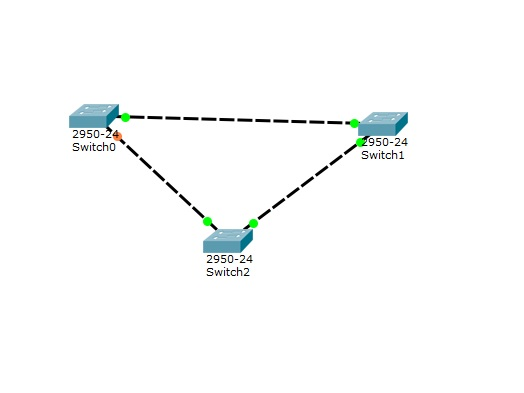
\includegraphics[width=0.90\textwidth]{./imagenes/red1}
	\caption{Red con bucle} 
\end{figure}
\vspace{7 cm}
\section{Actividad 2}
\begin{itemize}
\item En esta actividad configuramos el Switch 1 de la Figura 2.1 como primario y los demás como secundarios. Tal como se puede apreciar en la Figura 2.2 y 2.3

\vspace{1 cm}
\begin{figure}[h!]
	\centering
	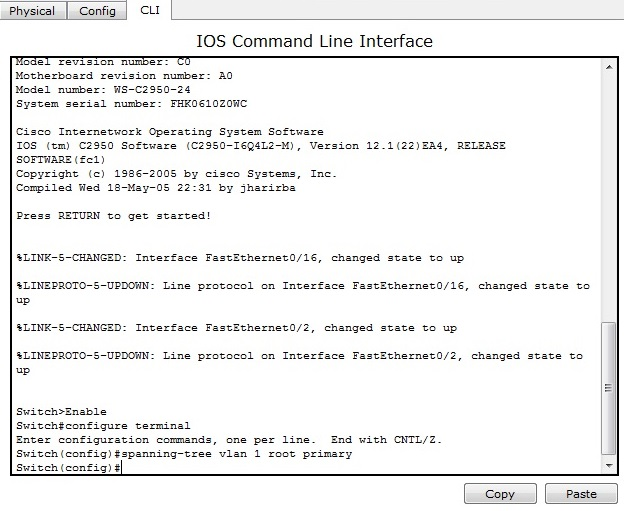
\includegraphics[width=0.90\textwidth]{./imagenes/red2}
	\caption{Configuracion del Switch 1} 
\end{figure}
\vspace{7 cm}
\item Aquí se configuro los otros Switches.\\
\begin{figure}[h!]
	\centering
	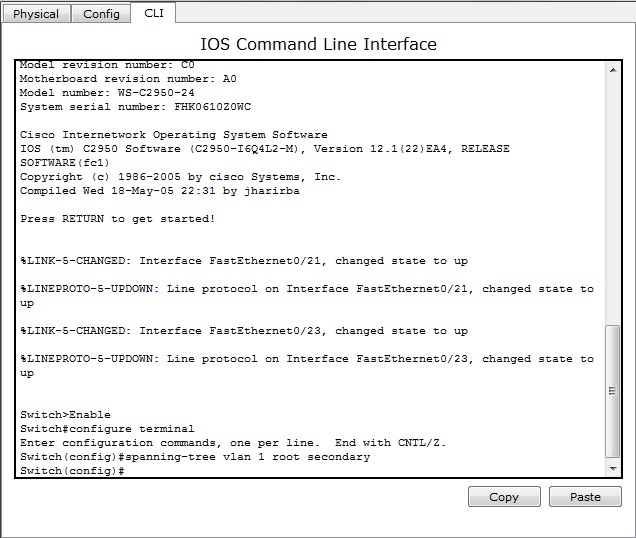
\includegraphics[width=0.90\textwidth]{./imagenes/redes3}
	\caption{Configuracion del Switch 0 y 2} 
\end{figure}
\end{itemize}
\vspace{8 cm}
\section{Actividad 3}
\begin{itemize}
\item Aquí se asignó la prioridad de cada Switch. Ver Figura 2.4 \\

\begin{figure}[h!]
	\centering
	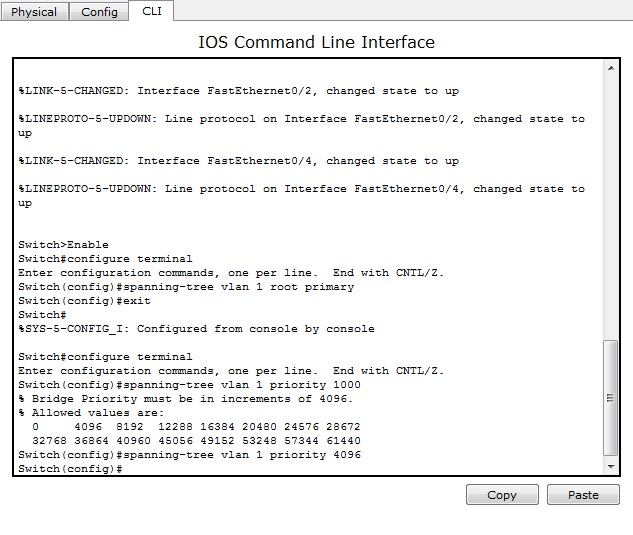
\includegraphics[width=0.90\textwidth]{./imagenes/redes4}
	\caption{Asiganción de prioridades de los Switches} 
\end{figure}


\end{itemize}
\vspace{8 cm}
\section{Preguntas Propuestas I:}
\subsection{(Activida I)¿Qué camino realizara un paquete que para llegar desde el switch
0 hasta el switch2?}
\begin{itemize}
\smallskip
\item Se envia el paquete al switch 2 y al switch 1, después el Switch 1 envía el paquete al Switch 2 y el Switch 2 envía el paquete al Switch 1, y asi sucesivamente creando un bucle.
\end{itemize}
\subsection{(Actividad I)¿Qué camino realizara un paquete que para llegar desde el switch
2 hasta el switch 1?}
\begin{itemize}
\item Se creara y se enviara directamente al Switch 1, por el cable que une el Switch 1 con el Switch 2
\end{itemize}
\subsection{(Actividad II)¿Qué camino realizara un paquete que para llegar desde el switch
2 hasta el switch 0?}
\begin{itemize}
\item Primero el paquete parte del switch 0 hasta el switch 1, y luego el paquete viaja del switch 1 hasta llegar al switch 2.
\end{itemize}
\subsection{(Actividad II)¿Qué camino realizara un paquete que para llegar desde el switch
1 hasta el switch 0?}
\begin{itemize}
\item Llega directamente al switch 0 ya que el switch 1 es el switch principal y el switch 0 es secundario.
\end{itemize}
\section{Actividad 4}
\begin{itemize}
\item En esta activad realizamos la topología de la Figura 2.5
\begin{figure}[h!]
	\centering
	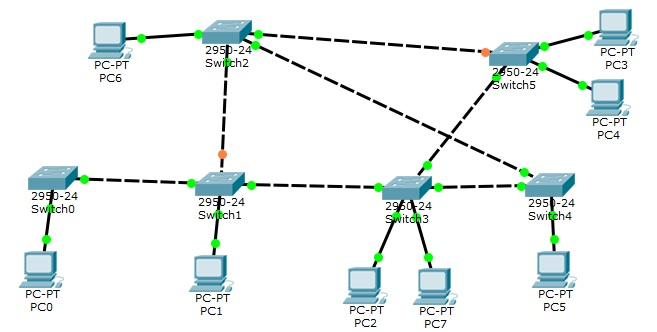
\includegraphics[width=0.90\textwidth]{./imagenes/redes6}
	\caption{Topología de la actividad 4} 
\end{figure}
\vspace{2 cm}
\item Configuramos los equipos con respecto al Cuadro 2.1.

\begin{table}[htbp]
\begin{center}
\begin{tabular}{| c| |c| |c| |c| |c|}
\hline
\multicolumn{5}{|c|}{VLANs} \\ \hline
Equipos & VLAN1 & VLAN2 & VLAN3 & VLAN4\\
\hline \hline
PC0 & X &   &   &  \\ \hline
PC1 &  & X  &   &  \\ \hline
PC2 &  &  &   & X \\ \hline
PC3 &  &  & X & \\ \hline
PC4 &  &  &  & X \\ \hline
PC5 &  &X  &  & \\ \hline
PC6 &  &  & X  & \\ \hline
PC7 & X & &  &  \\ \hline
\end{tabular}
\caption{Información de VLANs.}
\label{tabla:sencilla}
\end{center}
\end{table}

\item Configuramos los puertos de los switches, tal como aparece en la Figura 2.6.
\begin{figure}[htbp]
\centering
\subfigure[Configuracion de los puertos Access]{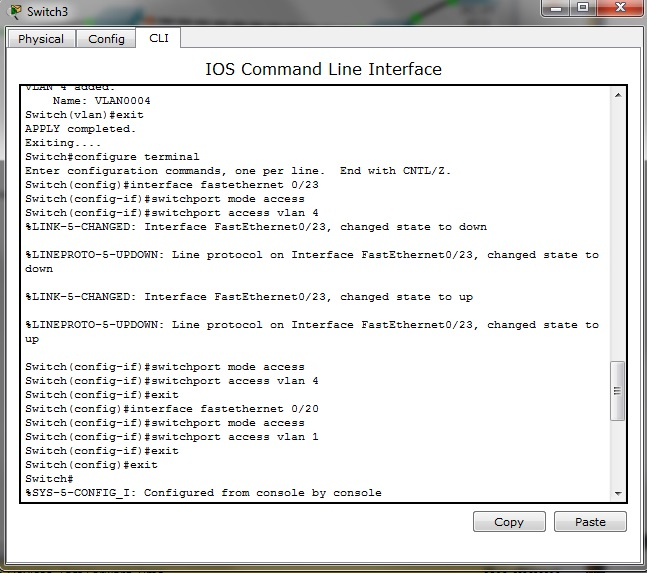
\includegraphics[width=82mm]{./imagenes/redes_7}}
\subfigure[Configuracion de los puertos Trunk]{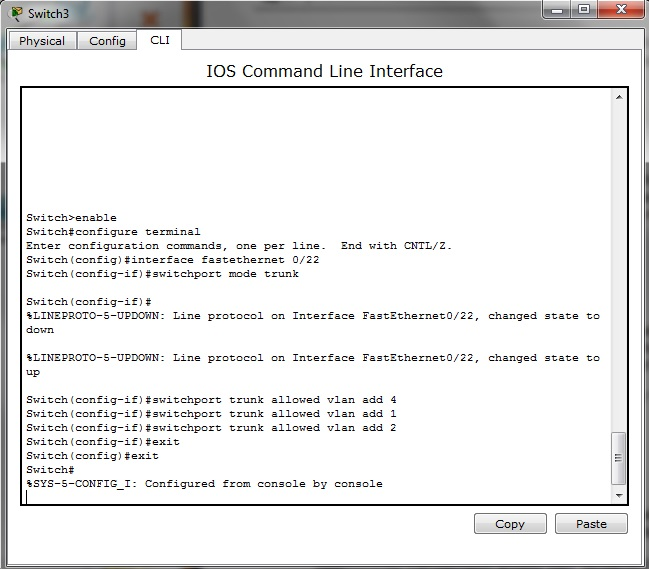
\includegraphics[width=82mm]{./imagenes/redes8}}
\caption{Configuracion del Switch 3.} 
\end{figure}
\vspace{7 cm}
\item También configuramos las IPs de cada computador como se puede apreciar en el cuadro 2.2



\begin{table}[h!]
\begin{center}
\begin{tabular}{| c| |c|}
\hline
\multicolumn{2}{|c|}{IPs} \\ \hline
Equipos & IP\\
\hline \hline
PC0 & 10.0.0.8  \\ \hline
PC1 & 10.0.0.2 \\ \hline
PC2 & 10.0.0.3  \\ \hline
PC3 & 10.0.0.7 \\ \hline
PC4 & 10.0.0.6  \\ \hline
PC5 & 10.0.0.5 \\ \hline
PC6 & 10.0.0.1  \\ \hline
PC7 &  10.0.0.4 \\ \hline
\end{tabular}
\caption{IP de cada PC.}
\label{tabla:sencilla}
\end{center}
\end{table}

%figura

\end{itemize}

\section{Actividad Propuestas II}
\subsection{¿Cuál es la diferencia del modo Access y el modo Trunk en un switch? }
\begin{itemize}
\item 
En el modo Access los puertos solo  transportan tráfico de una sola VLAN, la principal utilidad que se les da es conectar equipos finales. En cambio el modo Trunk puede transportar tráfico de múltiples VLANs, por lo que podemos tener múltiples VLANs en los switches y solo un enlace para transportar todo el tráfico.
\end{itemize}
\subsection{¿Qué ocurre si conecto una puerta en modo Trunk a un PC?}
\begin{itemize}
\item
Si se conecta una puerta en modo Trunk a un PC, funciona de igual manera que en modo Access, aunque no es recomendable, ya que el enlace pierde su funcionalidad troncal.
\end{itemize}
\subsection{¿Qué ocurre si conecto dos switches, uno en modo access y otro en modo trunk?}
\begin{itemize}
\item
Al conectar dos switches, uno en modo access y otro en modo trunk, el switch en modo access utilizaria N puertos para transportar N VLANs diferentes.
\end{itemize}
\subsection{¿Qué camino realizara un paquete que para llegar desde el switch 1 hasta el
switch 0?}
\begin{itemize}
\item
El paquete al momento de salir del switch 1 ingresa al enlace troncal en direccion al switch 0, luego llega a su destino al switch 0.
\end{itemize}



\chapter{Conclusión}
Como resultado del laboratorio realizado, pudimos entender con profundidad cómo funciona el protocolo STP y cuáles son las reglas que este sigue para ver que puertos van a estar designados o no, sin olvidar la importancia que posee, especialmente cuando se trata de una red con una alta redundancia de enlaces, los cuales son necesarios en muchos casos para garantizar la disponibilidad de las conexiones. Además, analizamos las distintas ventajas que poseen las redes VLAN en una topología y pudimos concluir que estas pueden ser de vital importancia en una organización, ya que pueden proporcionar seguridad cuando se trata con datos sensibles, reducir costos debido a la poca necesidad de actualizaciones caras y mejorar el rendimiento debido a la división de múltiples grupos lógicos de trabajo (dominio de broadcast) entre otros.

\section{Bibliografia}
\begin{itemize}
\item http://cisco.utmetropolitana.edu.mx/
\end{itemize}

\listoffigures


\end{document}